\documentclass[12pt,a4paper]{article}
\usepackage{preamble}


\PassOptionsToPackage{
  backend=biber,
  style=numeric, % eller authoryear
  sorting=nyt,
  giveninits=true,
  maxbibnames=99,
  doi=false,isbn=false,url=true,
  dashed=false
}{biblatex}


\usepackage{preamble}
\usepackage{xcolor}
\usepackage{booktabs}
\usepackage{circuitikz}
\usepackage{float} % for [H] exact figure placement
\usetikzlibrary{arrows.meta}

\usepackage{pgfplots}
\pgfplotsset{compat=1.18}



\addbibresource{./referanser.bib}

% ------ Metadata ------
\newcommand{\institution}{FHS/Cyberingeniørskolen}
\newcommand{\laboratory}{Elektronikklaboratoriet}
\newcommand{\coursecode}{INGXXXX \; XXXXXX}
\newcommand{\assignmentno}{H02}
\newcommand{\assignmenttype}{LABORATORIEXXXX}
\newcommand{\assignmenttitle}{XXXXXXXXXXXXXXXX}
\newcommand{\studentname}{Tor Johan Aleksandersen}
\newcommand{\partnername}{Morten Cleveland}
\newcommand{\class}{VING 78}
\newcommand{\labdate}{28.10.2025}
\newcommand{\submissiondate}{\today}

\begin{document}

\input{frontpage}

\pagenumbering{Roman}
\setcounter{page}{1}

\section*{Sammendrag}

Denne laboratorieøvelsen hadde som formål å undersøke og anvende maske- og nodeanalyse for å beregne strømmer og spenninger i motstandsnettverk med uavhengige spenningskilder, samt å studere funksjonen til en Wheatstone-målebru. For krets 1 og 2 ble teoretiske verdier bestemt ved hjelp av Kirchhoffs lover, og disse ble sammenlignet med praktiske målinger gjennomført med digitalt multimeter. Resultatene viste gjennomgående små avvik, hovedsakelig under $1\%$, noe som er i tråd med motstandenes toleranser og forventet måleusikkerhet. Krets 3 demonstrerte hvordan Wheatstone-broen kan balanseres og hvordan små variasjoner i motstandsforhold gir utslag i utgangsspenningen. Her ble spesielt den høye følsomheten nær balansepunktet tydelig observert. Identifiserte avvik ble forklart gjennom feilkilder som kontaktmotstand, kildevariasjoner og instrumentoppløsning. Øvelsen ga dermed både teoretisk og praktisk forståelse av kretsanalysemetoder og viste hvordan Wheatstone-broen kan benyttes i presisjonsmåling og sensorsystemer.
\clearpage

\tableofcontents
\clearpage

\pagenumbering{arabic}
\setcounter{page}{1}

\section{Innledning}

Denne rapporten vil undersøke hvordan maske- og nodeanalyse brukes til å beregne strømmer og spenningspotensialer i kretser, og hvordan Wheatstones målebru kan utnyttes til å omsette små resistansendringer til en målbar spenningsforskjell. Formålet vil være å belyse prinsippene bak metodene og å demonstrere dem eksperimentelt på enkle motstandsnettverk og en standard målebru. \\ Arbeidets omfang vil inkludere forbedrende beregninger, laboratoriemålinger på oppkoblede kretser, og en sammenligning mellom teoretiske resultater og praktiske måledata. Rapporten vil presentere diskusjon av funnene.
\clearpage

\section{Instrument- og komponentliste}

\subsection{Instrumentliste}
\begin{table}[h]
    \centering
    \caption{Instrumentliste}
    \label{tab:instrumentliste}
    \begin{tabular}{|l|l|l|c|}
        \hline
        \rowcolor[gray]{0.9}
        \textbf{Instrument} & \textbf{Beskrivelse} & \textbf{Serie Nr.} & \textbf{Antall} \\ \hline
        Instrument 1 & Multimeter          & xxxx & 1 \\ \hline
        Instrument 2 & Digitalt Multimeter  & xxxx & 1 \\ \hline
        Instrument 3 & Oscilloskop          & xxxx & 1 \\ \hline
        Instrument 4 & Telekombrett         & xxxx & 1 \\ \hline
        Instrument 5 & Strømforsyning       & xxxx & 1 \\ \hline
    \end{tabular}
\end{table}

\subsection{Komponentliste}
\begin{table}[h]
    \centering
    \caption{Komponentliste}
    \label{tab:komponentliste}
    \begin{tabular}{|l|l|c|}
        \hline
        \rowcolor[gray]{0.9}
        \textbf{Komponenttype} & \textbf{Verdi} & \textbf{Antall} \\ \hline
        Motstand             & 1k $\Omega$        & 1 \\ \hline
        Motstand             & 12k $\Omega$       & 1 \\ \hline
        Kobbertråd           & $\varnothing$0.9mm & 0.1m \\ \hline
        Variabel Kondensator & 4 -- 40 $pF$       & 1 \\ \hline
        Kondensator          & 220 $nF$           & 1 \\ \hline
        Isolert kobbertråd   & 4mm$^2$            & 1m \\ \hline
    \end{tabular}
\end{table}

\clearpage

\section{Teori}

\subsection{Formål og bakgrunn}
Formålet med denne laboratorieøvelsen er å belyse prinsippene bak maskeanalyse og nodeanalyse. 
Det gjennomføres beregninger av gitte kretser ved bruk av begge metodene, for deretter å bekrefte resultatene eksperimentelt i laboratoriet. 
Videre skal øvelsen gi en praktisk forståelse av hvordan en Wheatstones målebru fungerer, og hvordan lineære potensiometre og temperaturavhengige motstander kan påvirke stabiliteten i broen.



\subsection{Teoretisk grunnlag}
Det teoretiske grunnlaget i både maske- og nodeanalyse kommer fra teorien bak ohms lov og Kirchhoffs lover.



\subsubsection{Ohms lov}
\label{paragraph:OhmsLov}

Ohms lov beskriver sammenhengen mellom spenning, strøm og motstand i en elektrisk krets. 
Den sier at strømmen gjennom en metallisk leder med konstant temperatur er proporsjonal med den elektriske potensialforskjellen (spenningen) over lederen \cite{wikipediaOhmsLov}. 
Den matematiske formuleringen av Ohms lov er:
\[
I = \frac{V}{R}, \qquad V = IR
\]
der $I$ er strømmen gjennom lederen, målt i ampere $[A]$, $V$ er potensialforskjellen (spenningen) over lederen, målt i volt $[V]$, og $R$ er motstanden (resistansen), målt i ohm $[\Omega]$. 

Figuren under viser en enkel krets der alle disse størrelsene inngår.

\begin{figure}[H]
\centering
\begin{circuitikz}[american voltages]
    \node[circle, draw=black, fill=none, thick, inner sep=2pt] (A) at (-1,2) {};
    \node[circle, fill=black, inner sep=1.2pt] (B) at (1,2) {};
    \node[circle, fill=black, inner sep=1.2pt] (C) at (1,-2) {};
    \node[circle, draw=black, fill=none, thick, inner sep=2pt] (D) at (-1,-2) {};

    \node at (-1, 1.6) {$+$};
    \node at (-1, -1.6) {$-$};
    \node at (-1, 0) {$V$};

    \draw (A) to[short, -, i^=$I$] (B);
    \draw (B) to[R=$R$] (C);
    \draw (C) to[short, -] (D);
    

\end{circuitikz}
\caption{Illustrasjon av Ohms lov i en enkel krets.}
\label{fig:ohmsLov}
\end{figure}

\paragraph{Anvendelse av Ohms lov i kretsanalyse}

Ohms lov utgjør grunnlaget for analyse av elektriske kretser. 
Ved å kombinere loven med Kirchhoffs spennings- og strømlover kan man bestemme ukjente strømmer og spenninger i komplekse nettverk. 
I praksis brukes Ohms lov til å beregne spenningen over, strømmen gjennom eller motstanden til et element når to av størrelsene er kjent. 
For eksempel kan loven brukes til å verifisere målte verdier fra laboratorieforsøk og kontrollere om komponentene oppfører seg lineært innenfor sitt spesifiserte område.



\subsubsection{Kirchhoffs lover}
Kirchhoffs lover er todelt og beskriver to forskjellige fenomen i kretsanalyse. Det er i hovedsak to regler for konservering av elektrisk ladning og elektrisk energi i strømkretser. Kirchhoffs lover er sentrale i kretselektronikk fordi det brukes for å finne forholdet mellom strøm og spenning. De to reglene refereres som \textbf{Kirchhoffs strømlov} og \textbf{Kirchhoffs spenningslov} \cite{wikipediaKirchhoffsLover}.

\paragraph{Kirchhoffs strømlov.}
\label{paragraph:KCL}
Denne loven beskriver prinsippet om konservering av elektrisk ladning i et forgreningspunkt: "I et forgreningspunkt er summen av alle inngående strømmer lik summen av alle utgående strømmer." \cite{wikipediaKirchhoffsLover}. Matematisk kan det beskrives følgende:
\[
\sum_{n=1}^{N}I_n=0, \qquad \text{forgrening med \textit{N} grener}
\]

\noindent
Figuren under viser et enkelt tilfelle av et forgreningspunkt. Her vil $i_2+i_3=i_1+i_4$.

\begin{figure}[H]
\centering
\begin{circuitikz}[american voltages]
    \node[circle, fill=black, inner sep=1.2pt] (A) at (0, 0) {};
    \node[circle, fill=black, inner sep=1.2pt] (B) at (0, 3) {};
    \node[circle, fill=black, inner sep=1.2pt] (C) at (3, 0) {};
    \node[circle, fill=black, inner sep=1.2pt] (D) at (0, -3) {};
    \node[circle, fill=black, inner sep=1.2pt] (E) at (-3, 0) {};


    \draw (A) to[R=$R_1$, i^=$i_1$] (B);
    \draw (C) to[short, -, i^=$i_2$] (A);
    \draw (D) to[R=$R_3$, i^=$i_3$] (A);
    \draw (A) to[short, -, i^=$i_4$] (E);
    

\end{circuitikz}
\caption{Illustrasjon av et forgreningspunkt.}
\label{fig:KCL}
\end{figure}

\paragraph{Kirchhoffs spenningslov.}
\label{paragraph:KVL}
Denne loven beskriver konservering av elektrisk energi og sier at: "Summen av alle elektriske potensialforskjeller (spenninger) i enhver lukket strømsløyfe er lik null" og kan matematisk uttrykkes som:
\[
\sum_{n=1}^{N} V_n = 0, \qquad \text{Sløyfe med \textit{N} forgreninger}
\]

\noindent
I kretser vil dette i praksis bety at positive potensialforskjeller over batterier må veies opp av negative potensialforskjeller over motstander eller andre komponenter. Figuren under viser et enkelt tilfelle av en sløyfe der $V_1 + V_2 + V_3 = V_4$.

\begin{figure}[H]
\centering
\begin{circuitikz}[american voltages]
    \node[circle, fill=black, inner sep=1.2pt] (A) at (-3, 2) {};
    \node[circle, fill=black, inner sep=1.2pt] (B) at (3, 2) {};
    \node[circle, fill=black, inner sep=1.2pt] (C) at (3, -2) {};
    \node[circle, fill=black, inner sep=1.2pt] (D) at (-3, -2) {};


    \draw (A) to[R=$R_1$] (B);
    \draw (B) to[R=$R_2$] (C);
    \draw (C) to[R=$R_3$] (D);

    \node at (0, 1.4) {$V_1$};
    \node at (2.3, 0) {$V_2$};
    \node at (0, -1.4) {$V_3$};

    \draw (A) to[V=$V_4$] (D);

    

\end{circuitikz}
\caption{Illustrasjon av en sløyfe.}
\label{fig:KVL}
\end{figure}



\subsubsection{Nodal analyse}

Prinsippet for nodeanalyse bygger direkte på Kirchhoffs strømlov \ref{paragraph:KCL} og Ohms lov \ref{paragraph:OhmsLov}. 
Ved hjelp av disse lovene kombinert sammen kan man sette opp ligninger for ukjente spenninger i en krets. 
Nodeanalyse baserer seg på at summen av alle strømmer som går \emph{inn} i et forgreningspunkt (node) er lik summen av alle strømmer som går \emph{ut} fra noden. 
Med Ohms lov kan dette uttrykkes som:
\[
\sum_{n=1}^{N} I_n = 0, \qquad I = \frac{V}{R}
\]

\begin{figure}[H]
\centering
\begin{circuitikz}
    % Node in the center
    \node[circle, fill=black, inner sep=1.2pt, label=above right:$V_A$] (A) at (0,0) {};
    
    % Define outer connection points
    \node[label=left:$V_1$]  (L) at (-3,0) {};
    \node[label=right:$V_2$] (R) at (3,0) {};
    \node[label=above:$V_3$] (T) at (0,2) {};
    \node[label=below:$V_4$] (D) at (0,-2) {};
    
    % Draw resistors to each branch
    \draw (L) to[R=$R_1$, i>_=$I_1$] (A);
    \draw (R) to[R=$R_2$, i>_=$I_2$] (A);
    \draw (T) to[R=$R_3$, i<_=$I_3$] (A);
    \draw (D) to[R=$R_4$, i<_=$I_4$] (A);
\end{circuitikz}
\caption{Node med fire grener. Strømmer $I_1$ og $I_3$ går inn i noden, mens $I_2$ og $I_4$ går ut.}
\label{fig:node_analysis}
\end{figure}

\noindent
Figur \ref{fig:node_analysis} viser et forgreningspunkt med to inngående strømmer $I_1$ og $I_2$, og to utgående strømmer $I_3$ og $I_4$. Kirchhoffs strømlov gir formel:
\begin{equation}
    I_1 + I_2 = I_3 + I_4
    \label{eq:node_analysis_base}
\end{equation}

\noindent
Vi kan utlede denne ligningen videre med å ta hensyn til spenningsforskjell over respektiv motstand. Spenningsforskjellen over en komponent kan uttrykes som forskjellen i spenning før og etter, $V_{ab} = V_a - V_b$. Det betyr at vi kan videreutforme ligning \ref{eq:node_analysis_base} som:
\[
\frac{V_1 - V_A}{R_1} + \frac{V_2 - V_A}{R_2} = \frac{V_A - V_3}{R_3} + \frac{V_A - V_4}{R_4} 
\]
\noindent
Denne fremgangsmåten kan utvides til flere noder for å etablere et lineært likningssystem som beskriver hele kretsen. 
Ved å løse disse likningene finner man de ukjente nodepotensialene og dermed alle strømmer i kretsen.




\subsubsection{Maskeanalyse}
Maskeanalyse bygger på prinsippene fra Kirchhoffs spenningslov \ref{paragraph:KVL} og Ohms lov \ref{paragraph:OhmsLov}. Vi kan derfor summere spenningen over en sløyfe med \textit{N} sløyfer slik:

\[
\sum_{n=1}^{N} V_n = 0, \qquad \sum_{n=1}^{N} I_nR_n = 0
\]

For å gjøre utføre maskeanalyse vil det være nødvendig å definere strømretninger innenfor de forskjellige sløyfene i en krets og ladninger ($+$ eller $-$) ved inngangsterminalene til komponenter. Under vil et eksempel for en to-sløyfe krets vise hvordan vi kan definere slike terminalladninger og strømretninger.


\begin{figure}[H]
\centering
\begin{circuitikz}[american voltages]

    % --- Noder ---
    \node[circle, fill=black, inner sep=1.2pt] (A) at (-5,2) {};
    \node[circle, fill=black, inner sep=1.2pt] (B) at (0,2) {};
    \node[circle, fill=black, inner sep=1.2pt] (C) at (5,2) {};
    \node[circle, fill=black, inner sep=1.2pt] (D) at (5,-2) {};
    \node[circle, fill=black, inner sep=1.2pt] (E) at (0,-2) {};
    \node[circle, fill=black, inner sep=1.2pt] (F) at (-5,-2) {};


    % --- Komponenter ---
    \draw (A) to[R=$R_1$,*-] (B);
    \draw (B) to[R=$R_2$,-*] (C);
    \draw (B) to[R=$R_3$,*-*] (E);

    \node at (-3.4, 2.3) {$+$};
    \node at (-1.6, 2.3) {$-$};

    \node at (1.6, 2.3) {$+$};
    \node at (3.4, 2.3) {$-$};

    \node at (0.3, 0.9) {$+$};
    \node at (0.3, -0.9) {$-$};

    \draw (A) to[V=$V_1$, label position=right, *-*] (F);
    \draw (D) to[V=$V_2$, label position=left, *-*] (C);

    \draw (F) to[short,*-*] (E);
    \draw (E) to[short,*-*] (D);


    % --- Maske-strømmer (nå sentrert og runde) ---
    % Venstre maske
    \draw[->, very thick, >=Stealth] (-2.5,0) ++(0.9,0) arc (0:-330:0.9);
    \node at (-2.5,0) {$I_1$};

    % Høyre maske
    \draw[->, very thick, >=Stealth] (2.5,0) ++(0.9,0) arc (0:-330:0.9);
    \node at (2.5,0) {$I_2$};

\end{circuitikz}
\caption{To-sløyfe krets for maskeanalyse med maskestrømmene $I_1$ og $I_2$ (med klokka).}
\label{fig:mesh_two_loops}
\end{figure}

\noindent
Ved å følge strømmene i sløyfene og addere hver spenning over hver komponent kan vi uttrykke et likingssystem. Det lineære likningssystemet for denne kretsen vil være:

\begin{align}
    -V_1 + R_1I_1 + R_3(I_1-I_2) &= 0 \\
    -V_2 - R_3(I_1-I_2) + R_2I_2 &= 0
\end{align}

For hvert spenningsledd i sløyfen vi summerer vil fortegnet bestemmes av inngående terminals fortegn. I tilfellet der to strømmsløyfer inngår i én resistanse, ($R_3$ i figur \ref{fig:mesh_two_loops}) vil man summere strømmene med henholdsvis fortegn i retning av terminalene pluss ($+$) til minus ($-$).




\subsection{Wheatstone-bro}
En Wheatstone-bro er en elektrisk krets som er brukt for å måle en ukjent motstand. Metoden for dette er ved å balansere beinene i brokretsen. I tillegg har denne elektriske kretsen en fordel med å kunne gi ekstremt nøyaktige målinger i kontrast til en spenningsdeler. Wheatstonebroa er oppfunnet av Samuel Hunter Christie i 1833, men var forbedret og kjentgjort av Charles Wheatstone i 1843. \cite{wikipediaWheatstoneBridge}

\paragraph{Kretsen. } Kretsen til en Wheatstone-bro består av 2 parallellkoblet par av resistorer i seriekobling. I tillegg er det en spenningskilde. Dermed får vi to noder vi kan måle spenningen mellom for vår interesse. Dermed ser kretsen slik ut.

\begin{figure}[H]
\centering
\begin{circuitikz}[american voltages]

    % Diamond corners
    \node[circle, fill=black, inner sep = 1.2pt] (T) at (2,  2) {};  % top
    \node[circle, fill=black, inner sep = 1.2pt, label=left:$A$] (L) at (0, 0) {};  % left
    \node[circle, fill=black, inner sep = 1.2pt, label=right:$B$] (R) at ( 4, 0) {};  % right
    \node[circle, fill=black, inner sep = 1.2pt] (B) at (2, -2) {};  % bottom

    \node[circle, fill=black, inner sep = 1.2pt] (a) at (-4, 3) {};
    \node[circle, fill=black, inner sep = 1.2pt] (b) at (2, 3) {};
    \node[circle, fill=black, inner sep = 1.2pt] (c) at (2, -3) {};
    \node[circle, fill=black, inner sep = 1.2pt] (d) at (-4, -3) {};

    % Sides (use R for resistors; use short for just an outline)
    \draw (T) to[R, l_=$R_1$] (L);
    \draw (T) to[R=$R_2$] (R);
    \draw (B) to[R=$R_3$] (L);
    \draw (B) to[R, l_=$R_4$] (R);

    \draw (a) to[short,*-*] (b);
    \draw (b) to[short,*-*] (T);
    \draw (B) to[short,*-*] (c);
    \draw (c) to[short,*-*] (d);
    \draw (a) to[V=$V_{in}$] (d);

    \draw (L) to[voltmeter=$V_{out}$] (R);

\end{circuitikz}
\caption{Wheatstone-bro}
\label{fig:wheatstone_bridge}
\end{figure}

\paragraph{Utledning av formel ved balansert bro.}
I tilfellet av en balansert bro kan vi bruke Kirchhoffs strømlov \ref{paragraph:KCL} og Kirchhoffs spenningslov \ref{paragraph:KVL} for å utlede en formel for $V_{out}$. Definerer vi en strøm $I_G$ som går fra $A$ til $B$ kan vi sette opp Kirchhoffs strømlov i node $A$ og $B$ henholdsvis:
\[
I_1 = I_G + I_3
\]
\[
I_2 + I_G = I_4
\]
\noindent
Deretter, ved bruk av Kirchhoffs spenningslov kan vi sette opp to strømsløyfer med klokka. I øvre sløyfe har vi $I_T$ og i nedre har vi $I_B$.
\[
-R_1(I_T) + R_2(I_T) - R_G(I_B - I_T) = 0
\]
\[
+ R_G(I_B - I_T) + R_4(I_B) - R_3(I_B) = 0
\]
Strømmen som går gjennom $R_G$ må være $0$ i en balansert bro. Som betyr at $I_B - I_T = 0$. Ligningsystemet kan skrives som:
\begin{align}
    R_2 \cdot I_T &= R_1 \cdot I_T \label{eq:l1_wheatstone} \\
    R_4 \cdot I_B &= R_3 \cdot I_B \label{eq:l2_wheatstone}
\end{align}

\noindent
Ligning \ref{eq:l1_wheatstone} deles på \ref{eq:l2_wheatstone} og vi får:

\[
R_4 = \frac{R_3 \cdot I_B \cdot R_2 \cdot I_T}{I_B \cdot R_1 \cdot I_T}
\]
\begin{equation}
    \frac{R_4}{R_2} = \frac{R_3}{R_1} \qquad \rightarrow \qquad \frac{R_1}{R_3} = \frac{R_2}{R_4}
    \label{eq:balansertWheatstoneBro}
\end{equation}


\noindent
\paragraph{Utledning av $V_{out}$ i balansert bro.}
Teorien om spenningsdeling \ref{paragraph:wikipediaWheatstoneBridge} sier at spenningen i node A og B i figur \ref{fig:wheatstone_bridge} kan skrives slik:
\[
V_A = V_{in} \left( \frac{R_3}{R_1+R_3} \right)
\]
\[
V_B = V_{in} \left( \frac{R_4}{R_2+R_4} \right)
\]
$V_{out}$ er definert som $V_A - V_B$:
\[
V_{out} = V_{in} \left( \frac{R_3}{R_1+R_3} \right) - V_{in} \left( \frac{R_4}{R_2+R_4} \right)
\]
\begin{equation}
V_{out} = V_{in} \left( \frac{R_3}{R_1+R_3} - \frac{R_4}{R_2+R_4} \right)
\label{eq:spenning_i_wheatstone}
\end{equation}

\noindent
Ligning \ref{eq:spenning_i_wheatstone} er den endelige utledningen av spenningspotensialforskjellen i en Wheatstone-bro.



\subsubsection{Spenningsdeling og balanserte kretser}
\label{subsec:spenningsdeling}

\begin{figure}[H]
\centering
\begin{circuitikz}[american voltages]
    \node [circle, fill=black, inner sep = 1.2pt, label=above:$V_{in}$] (A) at (-5, 0) {};
    \node [circle, fill=black, inner sep = 1.2pt] (B) at (0, 0) {};
    \node [circle, fill=black, inner sep = 1.2pt] (C) at (5, 0) {};

    \node [circle, fill=black, inner sep = 1.2pt, label=right:$V_{node}$] (D) at (0, -2) {};

    \draw (A) to[R=$R_L$] (B);
    \draw (B) to[R=$R_R$] (C);

    \draw (B) to[short, -] (D);
    \node[ground] (GND) at (C) {};

\end{circuitikz}
\caption{Spenningsdeler krets}
\label{fig:spenningsdeler}
\end{figure}

En ideell spenningsdeler med to seriemotstander $R_\mathrm{topp}$ og $R_\mathrm{bunn}$ tilført $V_{in}$ gir noden mellom dem spenningen
\[
V_\mathrm{node} = V_{in}\frac{R_R}{R_L+R_R}.
\]
Denne formelen brukes gjentatte ganger i kretsanalyse og er grunnlaget for utledningen av Wheatstone-broen. En Wheatstone-bro er \emph{balansert} når (ligning \ref{eq:balansertWheatstoneBro})
\[
\frac{R_1}{R_3}=\frac{R_2}{R_4},
\]
som er ekvivalent med at nodene har samme potensial, altså $V_{out}=0$. For ubalanse fås den kjente uttrykksformen (ligning \ref{eq:spenning_i_wheatstone})
\[
V_{out}=V_{in}\!\left(\frac{R_3}{R_1+R_3}-\frac{R_4}{R_2+R_4}\right).
\]
\paragraph{Følsomhet.}
Små endringer i én gren gir størst utslag når broen er nær balanse (bratteste helning rundt $V_{out}=0$), derfor er Wheatstone-broen velegnet til presis måling av små motstandsvariasjoner.

\subsubsection{Lineære potensiometre}
\label{subsec:potmeter}

Et lineært potensiometer har total motstand $R_P$ og en sleider (wiper) som deler motstanden i to: 
\[
R_\uparrow = \alpha R_P,\qquad R_\downarrow=(1-\alpha)R_P,\qquad \alpha\in[0,1].
\]
Potensiometret kan brukes på to måter:
\begin{enumerate}
  \item \textbf{Som spenningsdeler} (tre terminaler): noden ved sleideren får 
  \(
  V_\mathrm{wiper}=V_{in}\frac{R_\downarrow}{R_\uparrow+R_\downarrow}
  =V_{in}(1-\alpha).
  \)
  \item \textbf{Som variabel motstand} (rheostat, to terminaler): effektiv motstand er en funksjon av $\alpha$, typisk
  \(
  R(\alpha)=\alpha R_P
  \)
  (eller $(1-\alpha)R_P$ avhengig av hvilke terminaler som brukes).
\end{enumerate}

I denne rapporten modelleres potensiometre i Wheatstone-broen som \emph{variable motstander} $x$ i stedet for faste $R$ (rheostat-bruk). Setter vi for eksempel
\[
R_1=R,\quad R_2=x,\quad R_3=R,\quad R_4=x,
\]
får vi fra broformelen
\[
V_{out}(x)=V_{in}\!\left(\frac{R_3}{R_1+R_3}-\frac{R_4}{R_2+R_4}\right)
=V_{in}\!\left(\frac{R}{R+R}-\frac{x}{x+R}\right)
=V_{in}\frac{R-x}{R+x}.
\]
Skriver vi om med motsatt fortegn får vi varianten som brukes i plottet:
\[
V_{out}(x)=V_{in}\frac{x-R}{x+R}.
\]

\paragraph{Relevans for temperaturmåling.}
En temperaturavhengig motstand (PTC/NTC) oppfører seg som et potensiometer der \emph{temperatur} styrer $x$. Når én gren er referanse og den andre er sensor, gir en liten endring i $x(T)$ en målbar $\Delta V_{out}$ rundt balansepunktet.

\paragraph{Praktiske hensyn.}
\begin{itemize}
  \item \textbf{Linearitet}: lineær (B-taper) antas; logaritmisk (A-taper) er uegnet her.
  \item \textbf{Endestopp og wiper-motstand}: gir små, men merkbare feil nær $\alpha\approx0$ og $1$.
  \item \textbf{Lasting}: målte $V_{out}$ forutsetter høy inngangsimpedans på voltmeter/DAQ.
\end{itemize}




\subsection{Kretser}
\subsubsection{Krets 1}

\begin{figure}[H]
\centering
\begin{circuitikz}[american voltages]

    % Diamond corners
    \node[circle, fill=black, inner sep = 1.2pt, label=above left:$A$] (A) at (-5, 2) {};
    \node[circle, fill=black, inner sep = 1.2pt, label=above:$B$] (B) at (0, 2) {};
    \node[circle, fill=black, inner sep = 1.2pt, label=above right:$C$] (C) at ( 5, 2) {};
    \node[circle, fill=black, inner sep = 1.2pt] (F) at (-5, -2) {};
    \node[circle, fill=black, inner sep = 1.2pt] (E) at (0, -2) {};
    \node[circle, fill=black, inner sep = 1.2pt] (D) at (5, -2) {};

    \draw (A) to[V, a^=$V_1$, l_=$12\text{V}$, i>^=$I_{R1}$] (F);
    \draw (D) to[V, a^=$V_2$, l_=$12\text{V}$, i>^=$I_{R1}$] (C);

    \draw (A) to[R, a^=$R_1$, l_=$1.5\text{k}\Omega$, i>^=$I_{R1}$] (B);
    \draw (B) to[R, a^=$R_2$, l_=$1.5\text{k}\Omega$, i>^=$I_{R2}$] (C);
    \draw (B) to[R, a^=$R_3$, l_=$1.5\text{k}\Omega$, i>^=$I_{R3}$] (E);

    \draw (D) to[short,*-*] (E);
    \draw (E) to[short,*-*] (F);

    \draw (0, -2) node[ground]{}; 

\end{circuitikz}
\caption{Krets 1}
\label{fig:krets1}
\end{figure}

\paragraph{Maskeanalyse.} Ved å sette $I_1$ i venstre loop med klokka og $I_2$ i høyre loop med klokka, setter vi opp følgende likninger ved bruk av KVL:
\begin{equation}
    -12\text{V} + R_1(I_1) + R_3(I_1 - I_2) = 0
    \label{eq:maskeKrets1l1}
\end{equation}
\begin{equation}
    -12\text{V} - R_3(I_1 - I_2) + R_2(I_2) = 0
    \label{eq:maskeKrets1l2}
\end{equation}
Kjente verdier for $R_1$, $R_2$ og $R_3$ settes inn, og likningene løses for $I_1$ og $I_2$. Ligning \ref{eq:maskeKrets1l1} og \ref{eq:maskeKrets1l2} blir følgende:
\[
    3000\Omega(I_1) - 1500\Omega(I_2) = 12\text{V}
\]
\[
    3000\Omega(I_2) - 1500\Omega(I_1) = 12\text{V}
\]
Løsning av likningene gir:
\[
    I_1 = I_2 = 8\text{mA}
\]
\[
    I_{R1} = I_{R2} = 8\text{mA} \qquad I_{R3} = I_1 - I_2 = 0\text{mA}
\]
Spenningen for B uttrykkes ved å lese spenningsfallet fra A til B. Derfor blir spenningen i punkt A, B og C blir følgende: 
\[
    V_A = V_1 = 12\text{V}
\]
\[
    V_C = - V_2 = -12\text{V}
\]
\[
    V_B = V_A - R_1 \cdot I_{R1} = 12\text{V} - 1500\Omega \cdot 8\text{mA} = 0\text{V}
\]

\paragraph{Nodeanalyse.} \label{paragraph:nodeanalyse} For å beregne $I_{R1}$, $I_{R2}$ og $I_{R3}$ ved bruk av nodeanalyse trenger vi å sette opp Kirchhoffs strømlov (KCL) for node B i kretsen. Ved å sette bunn som felles jording ($0\text{V}$) setter vi opp følgende likning:
\[
    \frac{V_A-V_B}{R_1} = \frac{V_B-0\text{V}}{R_3} + \frac{V_B-V_C}{R_2}
\]
\begin{equation}
    \frac{12\text{V}-V_B}{1500\Omega} = \frac{V_B}{1500\Omega} + \frac{V_B+12\text{V}}{3000\Omega}
    \label{eq:KCLiB}
\end{equation}
\[
    V_B = 0\text{V}
\]
Ved å sette $V_B$ inn i likningene for $I_{R1}$, $I_{R2}$ og $I_{R3}$ får vi:
\begin{align}
    I_{R1} &= \frac{V_A - V_B}{R_1} = \frac{12\text{V} - 0\text{V}}{1500\Omega} = 8\text{mA} \\
    I_{R2} &= \frac{V_B - V_C}{R_2} = \frac{0\text{V} - (-12\text{V})}{1500\Omega} = 8\text{mA} \\
    I_{R3} &= \frac{V_B - 0\text{V}}{R_3} = \frac{0\text{V} - 0\text{V}}{1500\Omega} = 0\text{A} \\
\end{align}

\paragraph{Node B. }Spenningen i punkt B er $0\text{V}$. Dette er forventet da motstandene $R_1$ og $R_2$ har samme verdi, og spenningskilden på $12\text{V}$ er lik for begge sider av kretsen. Punkt B vil derfor være i midten av de to spenningskildene hvor den ene siden ha like stor positiv spenning som den andre siden har negativ spenning. Flyten av strøm vil derfor gå mellom spenningskildene og ingenting vil gå gjennom $R_3$. \\ Forholdet mellom resistorene er nødvendig for at spenningen i node B skal være $0\text{V}$. Det må være like stor spenning fra begge sider av noden for forsikre at strømmen flyter gjennom $R_1$ og $R_2$ uten å rømme gjennom $R_3$. For at spenning i node B skal være $0\text{V}$ må følgende forhold mellom resistorene være oppfylt:
\[
    R_1 = R_2, \qquad R_3 \; \epsilon \; \mathbb{R^+}
\]

\paragraph{Toleranse i resistansene.} En feilmargin på $\pm$1\% i resistansene vil påvirke spenningen i node B. For å finne det maksimale og minimale spenningsnivået i node B må vi se på hvordan spenningen oppfører seg over resistansene. Resistansene vil ha størrelseområde
\[
\begin{aligned}
    R_1 &\in [1485\Omega,\; 1515\Omega] \\
    R_2 &\in [1485\Omega,\; 1515\Omega] \\
    R_3 &\in [1485\Omega,\; 1515\Omega]
\end{aligned}
\]

Tilfelle med maksimum verdi i $V_B$ oppstår når spenningsfallet er minst over $R_1$ og størst over $R_2$. Dette er fordi spenningen over $R_1$ er positiv i forhold til node B, mens spenningen over $R_2$ er negativ i forhold til node B. Det vi også ønsker er å isolere noden mest mulig fra referansejording i bunn. Dermed konkluderer vi følgende:
\[
\begin{aligned}
    V_{B,\text{max}} &: \quad 
        R_1 = R_{1,\text{min}}, \;
        R_2 = R_{2,\text{max}}, \;
        R_3 = R_{3,\text{max}} \\[4pt]
    V_{B,\text{min}} &: \quad 
        R_1 = R_{1,\text{max}}, \;
        R_2 = R_{2,\text{min}}, \;
        R_3 = R_{3,\text{min}}
\end{aligned}
\]
Ved å sette inn verdiene i likningen for KCL i node B får vi to ligninger som kan løses for $V_{Bmax}$ og $V_{Bmin}$. i praksis blir dette maksimum og minimum verdi vi kan se i målinger. Resultatet skal ligge mellom disse to verdiene.
\[
    \frac{V_A-V_{Bmax}}{1485\Omega} = \frac{V_{Bmax}-0\text{V}}{1515\Omega} + \frac{V_{Bmax}+12\text{V}}{1500\Omega}
\]
\[
    \frac{V_A-V_{Bmin}}{1515\Omega} = \frac{V_{Bmin}-0\text{V}}{1485\Omega} + \frac{V_{Bmin}+12\text{V}}{1500\Omega}
\]
\begin{equation}
    V_{Bmax}=0.80\text{mV}, \qquad V_{Bmin}=-0.80\text{mV}
    \label{eq:VBminmax}
\end{equation}

\subsection{Krets 2}

\begin{figure}[H]
\centering
\begin{circuitikz}[american voltages]

    % Diamond corners
    \node[circle, fill=black, inner sep = 1.2pt, label=above left:$A$] (A) at (-5, 2) {};
    \node[circle, fill=black, inner sep = 1.2pt, label=above:$B$] (B) at (0, 2) {};
    \node[circle, fill=black, inner sep = 1.2pt, label=above right:$C$] (C) at ( 5, 2) {};
    \node[circle, fill=black, inner sep = 1.2pt] (F) at (-5, -2) {};
    \node[circle, fill=black, inner sep = 1.2pt] (E) at (0, -2) {};
    \node[circle, fill=black, inner sep = 1.2pt] (D) at (5, -2) {};

    \node[circle, fill=black, inner sep = 1.2pt] (TL) at (-5, 4) {};
    \node[circle, fill=black, inner sep = 1.2pt] (TR) at (5, 4) {};


    \draw (A) to[V, a^=$V_1$, l_=$12\text{V}$, i>^=$I_{R1}$] (F);
    \draw (D) to[V, a^=$V_2$, l_=$12\text{V}$, i>^=$I_{R1}$] (C);

    \draw (A) to[R, a^=$R_1$, l_=$1.5\text{k}\Omega$, i>^=$I_{R1}$] (B);
    \draw (B) to[R, a^=$R_2$, l_=$1.5\text{k}\Omega$, i>^=$I_{R2}$] (C);
    \draw (B) to[R, a^=$R_3$, l_=$1.5\text{k}\Omega$, i>^=$I_{R3}$] (E);

    \draw (D) to[short,*-*] (E);
    \draw (E) to[short,*-*] (F);

    \draw (TL) to[R, a^=$R_4$, l_=$3.9\text{k}\Omega$, i>^=$I_{R4}$] (TR);
    \draw (A) to[short,*-*] (TL);
    \draw (TR) to[short,*-*] (C);

    \draw (0, -2) node[ground]{}; 

\end{circuitikz}
\caption{Krets 2}
\label{fig:krets2}
\end{figure}





\subsubsection{Maskeanalyse.} Vi definerer strømmene i de tre loopene som $I_1$, $I_2$ og $I_3$, alle med klokka. Ved bruk av KVL setter vi opp følgende likninger:


\begin{align}
    -12\text{V} + 1500\Omega (I_1 - I_3) + 1500\Omega (I_1 - I_2) &= 0 \label{eq:loop1} \\
    3900\Omega \cdot I_3 - 1500\Omega (I_2 - I_3) - 1500\Omega (I_1 - I_3) &= 0 \label{eq:loop2} \\
    -12\text{V} - 1500\Omega (I_1 - I_2) + 1500\Omega (I_2 - I_3) &= 0 \label{eq:loop3}
\end{align}

Løsning av likningene \ref{eq:loop1}, \ref{eq:loop2} og \ref{eq:loop3} gir:

\[
I_1 = 14.15\text{mA}, \quad
I_2 = 14.15\text{mA}, \quad
I_3 = 6.15\text{mA}
\]

Strømmene $I_1$, $I_2$ og $I_3$ definerer $I_{R1}$, $I_{R2}$, $I_{R3}$, $I_{R4}$ og $I_{R5}$ som følger:
\[
I_{R1} = I_1 - I_3 = 8.0\text{mA}
\]
\[
I_{R2} = I_2 - I_3 = 8.0\text{mA}
\]
\[
I_{R3} = I_1 - I_2 = 0\text{A}
\]
\[
I_{R4} = I_3 = 6.15\text{mA}
\]

\paragraph{Spenningene i nodene A, B og C.} Spenningene kan uttrykkes på samme måte som i ligning \ref{eq:KCLiB} under \ref{paragraph:nodeanalyse}. Ettersom at grenen fra node A til C vil ikke utgjøre en forskjell på $V_A$ og $V_C$ sammenlignet med krets 1, vil spenningene i nodene A, B og C være de samme som i krets 1:
\[
V_A = 12\text{V}, \quad V_B = 0\text{V}, \quad V_C = -12\text{V}
\]

\subsection{Krets 3}

\begin{figure}[H]
\centering
\begin{circuitikz}[american voltages]

    \node[circle, fill=black, inner sep = 1.2pt] (A) at (-6,  -2) {};
    \node[circle, fill=black, inner sep = 1.2pt] (B) at (-6,  2) {};
    \node[circle, fill=black, inner sep = 1.2pt] (C) at (-5,  2) {};
    \node[circle, fill=black, inner sep = 1.2pt] (D) at (-5,  3) {};
    \node[circle, fill=black, inner sep = 1.2pt] (E) at (-5,  1) {};

    \node[circle, fill=black, inner sep = 1.2pt, label=above:$1$] (F) at (0,  3) {};
    \node[circle, fill=black, inner sep = 1.2pt, label=below:$2$] (G) at (0,  1) {};

    \node[circle, fill=black, inner sep = 1.2pt] (H) at (5,  2) {};
    \node[circle, fill=black, inner sep = 1.2pt] (I) at (5,  3) {};
    \node[circle, fill=black, inner sep = 1.2pt] (J) at (5,  1) {};
    \node[circle, fill=black, inner sep = 1.2pt] (K) at (6,  2) {};
    \node[circle, fill=black, inner sep = 1.2pt] (L) at (6,  -2) {};

    \draw (B) to[V, a^=$V_{in}$, l_=$12\text{V}$, i>^=$I_{R1}$] (A);
    \draw (K) to[short,*-*] (L);
    \draw (F) to[voltmeter=$V_{out}$] (G);

    \draw (A) node[ground]{};
    \draw (L) node[ground]{};
    \draw (B) to[short,*-*] (C);
    \draw (H) to[short,*-*] (K);

    \draw (C) to[short,*-*] (D);
    \draw (C) to[short,*-*] (E);

    \draw (H) to[short,*-*] (I);
    \draw (H) to[short,*-*] (J);

    \draw (D) to[R=$R_5$] (F);
    \draw (E) to[R=$R_7$] (G);

    \draw (F) to[R=$R_6$] (I);
    \draw (G) to[R=$R_8$] (J);



\end{circuitikz}
\caption{Wheatstone-bro}
\label{fig:krets3}
\end{figure}



Ligningen for spenningen i Wheatstone-broen er gitt som:
\begin{equation}
    V_{out} = V_{in} \cdot  \left(\frac{R_8}{R_7 + R_8} - \frac{R_6}{R_5 + R_6}\right)
    \label{eq:wheatstoneKrets3}
\end{equation}
Der $V_{out}$ er spenning mellom node 1 og 2 i broen. Når broen er balansert, vil $V_{out} = 0\text{V}$. Dette skjer når følgende forhold er oppfylt:
\[
\frac{R_8}{R_7 + R_8} = \frac{R_6}{R_5 + R_6}
\]
\[
R_5 = R_6 = R_7 = R_8
\]
\paragraph{Lineære potensiometre.} Vi undersøker hvordan temperatur kan måles ved hjelp av et resistivt måleprinsipp basert på temperaturavhengige motstander (PTC-motstander). Vi kan simulere slike motstandere med bruk av lineære potensiometre. En lineær potensiometer har en motstandsverdi som er proporsjonal med hvor mye av potensiometret som er vridd. Ved å sette opp en Wheatstone-bro med to lineære potensiometre, kan vi simulere en temperaturmåling. Når den ene potensiometren representerer en referansetemperatur og den andre representerer den målte temperaturen, vil broen være balansert ved referansetemperaturen. Når temperaturen endres, vil motstandsverdien i den målte potensiometren endres, noe som fører til en ubalanse i broen og dermed en målbar spenning $V_{out}$. \\ For å oppnå høyest mulig potensialforskjell mellom node 1 og 2 gjennom måling av $V_{out}$, bør potensiometerne plasseres slik at ligning \ref{eq:wheatstoneKrets3} kan få høyest mulig verdi. Plasserer vi begge potensiometerne før målenodene blir det fortsatt balanse. Derfor må de plasseres diagonalt i broen for å oppnå størst $|V_{out}|$. Vi bytter derfor ut $R_5$ og $R_8$ med potensiometre. Ligningen kan skrives følgende:
\[
V_{out} = V_{in} \cdot  \left(\frac{R_8}{R_7 + R_8} - \frac{R_6}{R_5 + R_6}\right), \qquad R_5 = R_6 = R_7 = R_8
\]
\[
V_{out}(x_{pot}) = V_{in} \cdot  \left(\frac{x_{pot}}{R + x_{pot}} - \frac{R}{x_{pot} + R}\right)
\]
\[
V_{out}(x_{pot}) = V_{in} \cdot  \left(\frac{x_{pot} - R}{R + x_{pot}} \right)
\]
\noindent
$V_{out}$ er nå en funksjon for $x_{pot}$ og vi kan plotte den.



\begin{figure}[H]
\centering
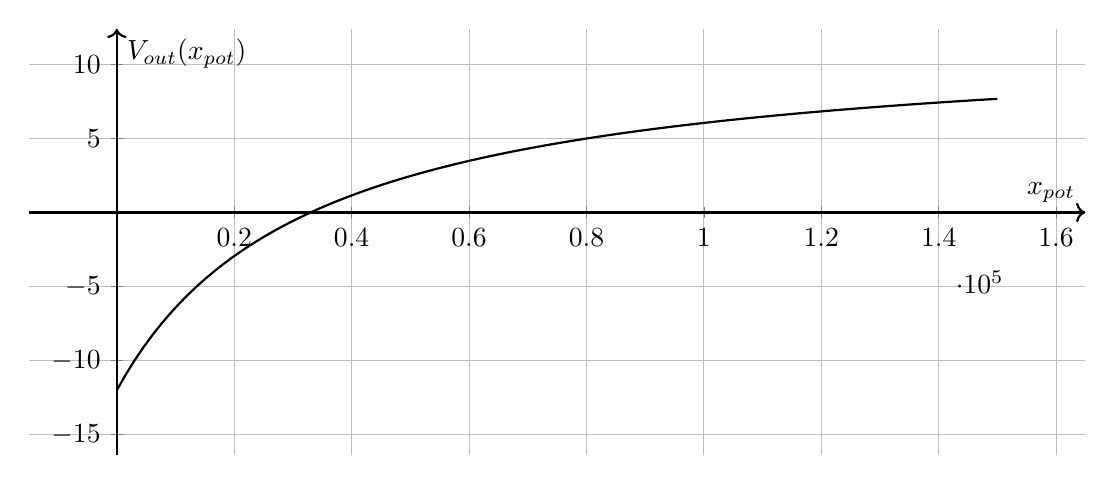
\begin{tikzpicture}
  \begin{axis}[
    xlabel=$x_{pot}$, 
    ylabel=$V_{out}(x_{pot})$,
    height=7cm,
    width=15cm,
    grid=both, 
    thick, 
    domain=0:150000, 
    samples=100, 
    ymin=-14, ymax = 10,
    axis lines=middle,           % move axes to the center (nice visual)
    axis line style={->},        % add arrows
    enlargelimits,               % small margin
  ]
    \addplot[black] {12 * ((x - 33000) / (x + 33000))};
  \end{axis}
\end{tikzpicture}
\caption{Graf}
\label{fig:wheatstone-graph}
\end{figure}

\vspace{1em}
\noindent
Grafens ekstremalpunkter i intervallet $x_{pot} \in [0, 100\text{k}\Omega]$ vil fortelle oss hva vi kan måle $V_{out}$ sin laveste og høyeste verdi vil være. Siden grafen oppfører seg som $V_{out}(s) < V_{out}(s + \Delta s)$ i intervallet $[0, 10^5]$ er den strengt økende og vi vil garantert finne dens laveste verdi i $x_{pot} = 0$ og høyest verdi i $x_{pot} = 10^5$. Dermed løser vi for det som:
\begin{align}
V_{out}(0) &= -12\text{V} \\
V_{out}(10^5) &= 6.05\text{V}
\end{align}
\clearpage

\section{Resultater}

\subsection{Krets 1}
\begin{table}[h!]
\centering
\begin{tabular}{lcc}
\toprule
\textbf{Komponent} & \textbf{Teoretisk verdi} & \textbf{Målt verdi} \\
\midrule
Strøm $I_{R1}$ & 8.00 mA & 7.95 mA \\
Strøm $I_{R2}$ & 8.00 mA & 8.10 mA \\
Strøm $I_{R3}$ & 0 A & 0.15 mA \\
Spenning $V_{A}$ & 12V & 12.01 V \\
Spenning $V_{B}$ & 0V & 0.028 V \\
Spenning $V_{C}$ & - 12V & -12.10 V \\

\bottomrule
\end{tabular}
\caption{Sammenlikning av teoretiske og målte verdier av komponenter i krets 1}
\label{tab:results1}
\end{table}

\subsection{Krets 2}
\begin{table}[h!]
\centering
\begin{tabular}{lcc}
\toprule
\textbf{Komponent} & \textbf{Teoretisk verdi} & \textbf{Målt verdi} \\
\midrule
Strøm $I_{R1}$ & 8.00 mA & 8.03 mA \\
Strøm $I_{R2}$ & 8.00 mA & 8.07 mA \\
Strøm $I_{R3}$ & 0 A & 0.021 mA \\
Strøm $I_{R4}$ & 6.15 mA & 6.21 mA \\
Spenning $V_{A}$ & 12V & 12.01 V \\
Spenning $V_{B}$ & 0V & 0.028 V \\
Spenning $V_{C}$ & - 12V & -12.09 V \\

\bottomrule
\end{tabular}
\caption{Sammenlikning av teoretiske og målte verdier av komponenter i krets 2}
\label{tab:results2}
\end{table}

\subsection{Krets 3}
\begin{table}[h!]
\centering
\begin{tabular}{lcc}
\toprule
\textbf{Komponent} & \textbf{Teoretisk verdi} & \textbf{Målt verdi} \\
\midrule
Spenning $V_{12}$ & 0 V & 6.5 mV \\
Spenning $V_{12} |_{min}$ & -12 V & -11.97 V \\
Spenning $V_{12} |_{maks}$ & 6.05 V & 6.47 V \\

\bottomrule
\end{tabular}
\caption{Sammenlikning av teoretiske og målte verdier av komponenter i krets 3}
\label{tab:results3}
\end{table}
\clearpage

\section{Diskusjon}

\subsection{Metode og måleforutsetninger}
I krets 1 benyttet vi både maskeanalyse og nodeanalyse for å beregne oss fram til ulike kjente verdier i et motstandsnettverk med uavhengige spenningskilder. Krets 2 er for det meste lik som krets 1, men her benyttet vi maskeanalyse for å sette opp maskelikningene. \\ Metoden for å utføre dette innebærer komponentene og instrumentene i figur \ref{tab:komponentliste} og \ref{tab:instrumentliste}. \\ De teoretiske verdiene som er presentert i teorien har blitt praktisk målt i laboratioriet for å bekrefte ulike ting ... . I denne rapporten vil vi kunne 



\subsection{Feilkilder}
Elektriske kretser er alltid forbundet med ulike feilkilder som kan påvirke måleresultatene. 
Disse feilkildene er hovedårsaken til at praktiske målinger ofte avviker noe fra teoretiske verdier. 
Selv når resultatene viser god overensstemmelse, vil mindre avvik kunne forklares gjennom slike faktorer. \\ I denne rapporten vurderes de mest relevante feilkildene for krets~1, krets~2 og krets~3. \\ De omfatter kontaktmotstand og dårlige koblinger, spenningskildens egenskaper, måleinstrumentets påvirkning, restspenninger i kretsen, samt generell måleusikkerhet og oppløsning. 

\paragraph{Kontaktmotstand og dårlige koblinger.}
\label{par:mo}
I koblingsbrett, ledninger og komponentoverganger vil kontaktmotstand oppstå. Kontaktmotstanden er den elektriske motstanden som oppstår i grenseflaten mellom to ledere som er koblet sammen \cite{wikipediaOhmsLov}. Denne vil være variabel i hver hvert kontaktpunkt og vil garantere ubalanser i målinger overalt i kretsen. Dårlige kontaktpunkter vil gi økt motstand, og dette særlig i lavstrømsgrener. \\ 
Ser vi på våre resultater i krets 1 (tabell \ref{tab:results1}) ser vi at de fleste målinger er innenfor $1\%$, men kontaktmotstand og dårlige koblinger kan forklare avvikket på $1.25\%$ i strøm $I_{R2}$.


\paragraph{Spenningskilden.}
I teoretiske utregninger antar vi at den interne motstanden i spenningskilden er lik null for simplisiteten av kretsen. Dette lager en reell feilkilde der det vil være en liten, ukjent indre motstand i spenningskildekomponenten. I tillegg vil spenningskilden ha små variasjoner i utgangsspenning over tid. Dette påvirker hvordan strømmen over motstand $R_1$ og $R_2$ vil variere og ikke være perfekt i forhold til den teoretiske utregningen. I tillegg kan vi trekke dette under nullspenningen i node B. Når de to uavhengige spenningskildene produserer inkonsise spenninger vil det påvirke spenningen i node B. I krets 3 kan vi se på formelen for $V_{out}$ (ligning \ref{eq:spenning_i_wheatstone}):

\[
V_{out} = V_{in} \left( \frac{R_3}{R_1+R_3} - \frac{R_4}{R_2+R_4} \right)
\]
\[
V_{out} = V_{in} \cdot x 
\]

\noindent
Her vil x representere det lineære forholdet mellom $V_{out}$ og $V_{in}$. Siden spenningskilden her er $V_{in}$ vil disse feilkildene påvirke $V_{out}$ proporsjonalt.


\paragraph{Måleinstrumentet.}
Multimeteret er ikke noe vi tar hensyn til i teoretiske utregninger siden det spiller ikke en rolle i en krets. Hensikten med et multimeter er å parallellkobles i to punkter av interesse, der multimeteret har en høy indre motstand for å ikke påvirke kretsen. Uansett, vil denne indre motstanden variere og oppløsningen på instrumentet vil forhindre de mest nøyaktige målingene. Dette kan ha innspill på målingene til en viss grad, og vi kan si at det er noe av grunnen til avvik i alle praktiske målinger.



\paragraph{Restspenninger.}
Restspenninger oppstår som grunn av kontaktmotstand og dårlige koblinger. Disse forskjellene i kontaktmotstander i koblingsbrettet og i hele laboratorieoppsettet vil lage små jordpotensialforskjeller. Dette vil i vårt tilfelle ha en direkte påvirkning på nullspenningen i node B, $V_B$, og det vil ha innvirkninger på hele kretsen i alle målinger.


\paragraph{Måleusikkerhet og oppløsning.}
Multimeteret vil ha en måleusikkerhets pågrunn av dens oppløsning i hva den kan måle. Dette bidrar til at små spenninger og strømmer har høy relativ feil. et multimeter med nøyaktighet $\pm 0.5\%$ gir usikkerhet på rundt $\pm 0.06\text{V}$ ved $12\text{V}$ måling. I tillegg for millivolt-nivåer (som $V_B = 0.028\text{V}$), er usikkerheten relativt sett svært stor. Dette vil påvirke resultatene våre på en dårlig måte. Noen avvik kan derfor ligge innenfor måleusikkerheten.

\vspace{1em}
\noindent
Samlet sett forklarer disse feilkildene de små, men målbare forskjellene mellom teoretiske og eksperimentelle verdier. De største bidragene antas å være kontaktmotstand og måleusikkerhet, mens variasjon i spenningskildene og restspenninger har mindre, men merkbar innvirkning på nøyaktigheten.







\subsection{Resultater knyttet til teori}

Dette delkapitlet sammenligner de målte verdiene fra laboratoriefosøket med de teoretiske beregnet utledet i kapittel \ref{sec:toeri}. Hensikten er å vurdere om resultatene følger de forventede sammenhengene Ohms lov, Kirchhoffs lover, og teorien for maske- og nodeanalyse samt Wheatstone-broen. Under vil det drøftes resultater opp mot teori for hver krets med feilkilder i fokus.
\subsubsection{Krets 1}
Metoden brukt her er maske- og node-analyse. Begge metodene gir $I_{R1} = I_{R2} = 8.00\text{mA}$ og $I_{R3} = 0\text{A}$. De målte resultatene varierer litt og gir alle litt avvik fra den teoretiske verdien. Strøm $I_{R2}$ avviker mest i hele tabell \ref{tab:results1} med over $1\%$, og resten under. Avviket i $I_{R1}$ kan forklares av flere feilkilder, som kontaktmotstand og dårlige koblinger. Andre feilkilder som spenningskilden vil også kunne spille inn her, da den kan produsere spenninger med feilmarginer. I tillegg kan vi se at i krets 1 er motstanden $R_1$ koblet i serie fra et nodepotensial $-12\text{V}$ i C til et nodepotensial $0\text{V}$ i B. Våre målinger for $V_C$ og $V_B$ samsvarer ikke med dette, og det vil være en grunn for at strømmen i $R_2$ har mye avvik. Vi kan trygt si at disse verdiene ligger innenfor en akseptabel avstand fra den teoretiske verdien. Tar vi for oss regnestykket for strømmen gjennom motstanden $R_2$ med de praktiske målingene får vi:
\[
I_{R2} = - \frac{V_C - V_B}{R_2}
\]
\[
I_{R2} = - \frac{-12.10\text{V} - 0.028\text{V}}{1500\Omega}
\]
\[
I_{R2} = 8.05\text{mA}
\]
\noindent
Dette viser at spenningen i node C vår bidrar til avviket. $V_C$ har allerede et avvik på $0.83\%$ som er ganske stort, men akseptabelt siden det ligger innenfor $1\%$. Denne målingen er tatt i parallell mellom selve spenningskilden ($-12\text{V}$) og jording ($0\text{V}$) og vil gjenspeile hva spenningskilden er stilt inn til. Derfor vil disse ujevne målingene direkte stamme fra spenningskilden og restspenninger som feilkilder. Samtidig kan vi trekke $V_B$ under dette fordi den bygger på relasjonen mellom spenningen i nodene A og C og motstandene mellom, som er utledet og presentert i ligning \ref{eq:KCLiB} som vist under. 
\[
\frac{V_A-V_B}{R_1} = \frac{V_B}{R_3} + \frac{V_B - V_C}{R_2}
\]
\noindent
Her ser vi tydelig at spenningen i node B vil avhenger av mange feilkilder som spiller inn på hvert enkeltelement i ligningen. I tillegg har hver motstand et feilmarginområde på $\pm 1\%$. Dette fører til et teoretisk usikkerhetsområde på $80\text{mV}$. Den praktiske målingen er $+ 28\text{mV}$. Målingen er innenfor godkjente rammer. \\ Vi trekke en konklusjon for målingene i krets 1 om at målingene ligger innenfor forsøkets satte godkjente grense på $1\%$ med noen unntak som kan forklares i grunnleggende kretsfeilkilder. 

\subsubsection{Krets 2}
Krets 2 bygger videre på krets 1, men med en ekstra gren via motstanden $R_4$ mellom node A og C. 
Teoretiske beregninger ved maskeanalyse ga $I_{R4}=6.15\text{mA}$, mens målingen viste $6.21\text{mA}$, et avvik på $0.98\%$. 
Dette er innenfor komponentenes toleranse på $\pm1\%$, og samsvarer derfor med teorien.

Sammenlignes strømverdiene i $R_1$ og $R_2$ mellom krets 1 og 2 (tabell~\ref{tab:results1}\ref{tab:results2}), ser vi at de holder seg nær identiske, begge rundt $8.0\text{mA}$. 
Dette viser at tilkoblingen av $R_4$ primært påvirker strømfordelingen mellom grenene A-C, uten å endre nodepotensialene $V_A$, $V_B$ og $V_C$ merkbart. Dette ser vi også i nodeanalyse for node B i teorien (ligning \ref{eq:KCLiB}):
\[
\frac{V_A-V_B}{R_1} = \frac{V_B}{R_3} + \frac{V_B - V_C}{R_2}
\]
\noindent
Derfor kan vi isolere oss til selve grenen mellom node A og C og se på strømmen. Små avvik mellom beregnet og målt strøm kan igjen forklares av kontaktmotstand og interne spenningskildevariasjoner (se avsnitt~\ref{par:mo}).

Spenningene i nodene viser også god overensstemmelse med teori. 
Node B har en målt spenning på $0.028\text{V}$, som er godt innenfor beregnet område $\pm 80\text{mV}$ fra ligning \ref{eq:VBminmax}. 
Avvikene mellom målt og teoretisk verdi er dermed konsistente med forventede feilkilder, og bekrefter at Kirchhoffs lover holder innenfor eksperimentell nøyaktighet.

\subsubsection{Krets 3}
I teorien utledet vi et uttrykk for spenningen i Wheatstone-broen (se ligning \ref{eq:spenning_i_wheatstone}). Med potensiometre modellert diagonalt i broen som henvist i teorien utledet vi uttrykket (se ligning \ref{eq:pot_i_wheatstone}):
\[
V_{out}(x) = V_{in}\frac{x - R}{x + R}
\]
\noindent
Denne gir maksimal følsomhet nær balansepunktet $\left( x \approx R \right)$. Ser vi på resultatene i tabell \ref{tab:results3} målte vi spenningen i broen til å være $6.5\text{mV}$, da den teoretiske verdien er $0\text{V}$ så er dette godt innafor. Komponentene som påvirker $V_{out}$ kan vi lese av ligning \ref{eq:spenning_i_wheatstone} til å være motstandene og spenningskilden i kretsen. Aktuelle feilkilder vil da være kontaktmotstand og dårlige koblinger i motstandene. Siden kretsen har fire slike motstander vil ubalansen påvirket av feilkildene bli større. I tillegg til at selve kildespenningen vil ha egne mulige feilkilder kan vi ikke lene oss på at $V_{in}$ i formelen er pålitelig heller. Restspenninger vil dannes i nodene i Wheatstone-broen og vil også påvirke målingen $V_{12}$. 
\\[1em]
Videre kan vi se på målingen $V_{12}|_{min}$ i tabell \ref{tab:results3} og den har et avvik på $0.25\%$ som er godt innafor. Siden dette er en spenningsmåling ser vi på de samme effektive feilkildene som i måling $V_{12}$. Videre mulige feilkilder vil tilknyttes potensiometerne i kretsen. Vi må se på uttrykket for $V_{out}(x)$, der $x$ er motstanden i begge potensiometerne. $V_{12}|_{min}$ innebærte å stille disse til $0$, potensiometerne er derfor ikke en veldig stor feilkilde utenom dens indre motstand. Målingen for $V_{12}|_{min}$ blir derfor nøyaktig. 
\\[1em] 
$V_{12}|_{maks}$ har et mye større og uakseptabelt avvik på $3.64\%$. Her må vi trekke fram de relevante feilkildene for å besvare dette. Den teoretiske verdien baserer seg på at begge potensiometerne har maksimummotstand på nøyaktig $10^5\Omega$, men det er ikke sikkert og derfor vil det bli en aktuell feilkilde i forsøket vårt. Ser vi på tilfelle hvor potensiometerne er i ubalanse på maksimumresistanse gir det mye utslag på den teoretiske $V_{out}$ i ligning \ref{eq:pot_i_wheatstone}:
\[
V_{out}(x_{pot}) = V_{in} \cdot  \left(\frac{x_{pot} - R}{R + x_{pot}} \right)
\]
\noindent
Hvis vi skal få $V_{out}$ til å nærme seg den praktiske målingen $6.27\text{V}$ må potensiometerne være lik verdi så vi kan fortsatt bruke ligningen over. For å finne $x_{pot}$ tar vi for oss regnestykket:
\begin{align}
  V_{out}(x_{pot}) &= 6.27\text{V} \\
  x_{pot} &= 105\,219.89\Omega
\end{align}
Dette presenterer at potensiometerne må begge ha en egentlig resistansefeilmargin på $+5.22\%$. Som er realistisk, men dette forutser at hele feilkilden ligger i akkurat dette momentet. Det er i tillegg til potensiometerresistansen de samme aktuelle feilkildene her som i måling av $V_{12}|_{min}$. Derfor kan vi påstå at målingen er realistisk, men med en uakseptabel avviksprosent.


\subsection{Hovedfunn opp mot hensikt}
Hensikten med forsøket var å belyse prinsippene bak maske- og nodeanalyse, samt studere hvordan en Wheatstone-målebru kan brukes til å måle små motstandsvariasjoner. 
Resultatene fra krets 1 og krets 2 viser at både maskeanalyse og nodeanalyse gir korrekte og konsistente teoretiske verdier for strømmer og nodepotensialer, der avvik kan forklares i grunn av feilkilder. 
De fleste praktiske målingene ligger innenfor forventede avvik basert på komponenttoleranser og måleusikkerhet, og noen ligger utforbi. Målinger som ligger utforbi har vært argumentert for med feilkilder. Uansett, så bekrefter de praktiske måledataene at metodene beskriver kretsene på en presis måte.
\\[1em]
For Wheatstone-broen i krets 3 ble det observert et restsignal nær balansepunktet, samt en tydelig endring i $V_{out}$ når forholdet mellom motstandene ble justert. Dette stemmer godt med den teoretiske modellen, og demonstrerer hvordan broen er spesielt følsom for små endringer i motstandsverdi rundt balansepunktet.
\\[1em]
Samlet sett viser forsøket at både maske- og nodeanalyse fungerer som pålitelige verktøy for kretsanalyse, og at Wheatstone-broen er velegnet for presis måling av små motstandsvariasjoner, slik forsøkshensikten beskriver.



\subsection{Mulige bruksområder}
Maske- og nodeanalyse brukes bredt innen analyse, design og feilsøking av elektriske kretser. 
Metodene danner grunnlaget for å bestemme strøm- og spenningsfordeling i alt fra enkle motstandsnettverk til mer komplekse signalbehandlings- og sensorkretser, og inngår som standard verktøy i både undervisning og industrirettet kretskonstruksjon \cite{aac_mesh, aac_node}.

Wheatstone-broen er spesielt nyttig når små endringer i motstand skal måles presist. 
Broen gjør det mulig å omsette svært små variasjoner i resistans til målbare spenningsendringer, og brukes derfor i et stort spekter av sensorer og målesystemer \cite{omega_wheatstone}. 
Typiske anvendelser inkluderer strekkmålere i vektceller, hvor mekanisk deformasjon påvirker motstanden, samt temperaturavhengige motstander (NTC/PTC) og trykk- eller posisjonssensorer. 
I slike systemer gir Wheatstone-broen høy følsomhet og god stabilitet, noe som gjør den egnet i presisjonsmåleinstrumenter og industrielle overvåkingsapplikasjoner.



\subsection{Forbedringer og videre arbeid}
En naturlig forbedring av forsøket ville være å måle de faktiske resistansverdiene til alle motstandene som inngår i kretsene. Dette ville gjort det mulig å beregne nye teoretiske strøm- og spenningsverdier med reelle komponentdata, og dermed undersøke om avvikene hovedsakelig skyldes toleranser eller andre feilkilder. Dette kunne også gitt et bedre grunnlag for å forklare avviket i $V_{12}|_{maks}$ i krets 3, ved å analysere uttrykket for $V_{out}(x_{pot})$ med potensiometerets faktiske motstandsverdi (se ligning \ref{eq:pot_i_wheatstone}).
\\[1em]
En annen forbedring ville være å karakterisere spenningskilden. I dette forsøket ble den interne motstanden og nøyaktigheten til kilden antatt, men ikke målt. Ved å måle kildeimpedans og faktisk utgangsspenning under last kunne mer presise simuleringer utføres, og avvikene i både krets 1 og 2 kunne vurderes mer nøyaktig.
\\[1em]
For Wheatstone-broen i krets 3 kunne forsøket vært utvidet ved å måle $V_{out}$ for flere posisjoner på potensiometeret og deretter plotte den praktiske kurven. En slik kurve kunne sammenlignes direkte med den teoretiske modellen vist i figur \ref{fig:wheatstone-graph}, og dette ville gitt innsikt i hvor følsom broen er nær balansepunktet og hvor avviket øker mot endeposisjonene.

\paragraph{Videre arbeid.}  
Dette forsøket har introdusert og anvendt prinsippene for både node- og maskeanalyse, samt demonstrert funksjonen til en Wheatstone-bro. Et naturlig videre arbeid vil være å anvende disse analysemetodene på mer komplekse nettverk, for eksempel kretser som inneholder forsterkere eller flere koblingsnoder, der systematisk kretsanalyse blir enda viktigere.
\\[1em]
Videre kunne Wheatstone-broen i krets 3 vært brukt som utgangspunkt for et mer praktisk målesystem. Wheatstone-broen brukes ofte i sensorer der små endringer i motstand må omsettes til målbare elektriske signaler, slik som i \textit{strain gauges} (strekkmålere) og vektceller \cite{omega_wheatstone}. Et aktuelt videre eksperiment kunne derfor vært å erstatte potensiometeret med en strekkmåler, og undersøke hvordan mekanisk deformasjon gir utslag i brospenningen. Dette ville gi en direkte kobling mellom teoretisk kretsanalyse og reelle, fysiske måleapplikasjoner.
\clearpage

\section{Konklusjon}
Formålet med forsøket var å belyse prinsippene bak maske- og nodeanalyse, i tillegg til å studere funksjonen til en Wheatstone-målebru. De praktiske måleresultatene samsvarer med teorien og viser at både maske- og nodeanalyse er pålitelige metoder for å analysere elektriske kretser. Avvikene er akseptable, men kan også forklares av feilkilder.
\\[1em]
Wheatstone-broen viste en tydelig sammenheng mellom ubalanse i motstandsforholdene og utgangsspenningen. Målingene viser at broen er mest følsom nær balansepunktet, slik teorien tilsier. Avvikene i maksimal utgangsspenning kan knyttes til praktiske forhold som internmotstand i spenningskilden og feilmargin i potensiometermotstanden.

Samlet sett oppfylte forsøket hensikten. Arbeidet ga både teoretisk og praktisk innsikt i hvordan elektriske kretsanalyser utføres, og hvordan Wheatstone-broen kan benyttes til nøyaktige resistansmålinger. Videre arbeid kan omfatte måling av faktiske komponentverdier, karakterisering av spenningskilde og måleinstrument, samt bruk av broen sammen med temperatur- eller streinmålesensorer i et komplett målesystem.
\clearpage

\nocite{*}
\printbibliography[heading=bibintoc,title={Referanser}]
\clearpage

\section*{Vedlegg}
\addcontentsline{toc}{section}{Vedlegg}
\input{sections/vedlegg}
\clearpage

\end{document}
